\documentclass[a4paper,10pt]{article}

\usepackage[utf8]{inputenc}
\usepackage[T1]{fontenc}
\usepackage[english]{babel}

\usepackage{color}
\usepackage{float}
\usepackage{fancyvrb}

\usepackage{amssymb}
\usepackage{amsmath}

\usepackage{listings}
\usepackage{comment}
\usepackage[boxed]{algorithm2e}
\usepackage{graphicx}
\usepackage{subcaption}
\usepackage{subfig}

\usepackage{amsthm}
\theoremstyle{plain}

\theoremstyle{definition}
\newtheorem{defn}{Definition}
% \begin{defn}Here is a new definition.\end{defn}

\DeclareGraphicsExtensions{.png}

\definecolor{dkgreen}{rgb}{0,0.45,0}
\definecolor{gray}{rgb}{0.5,0.5,0.5}
\definecolor{mauve}{rgb}{0.30,0,0.30}

\lstset{frame=tb,
  language=Java,
  aboveskip=3mm,
  belowskip=3mm,
  showstringspaces=false,
  columns=flexible,
  basicstyle={\small\ttfamily},
  numbers=left,
  numberstyle=\footnotesize,
  keywordstyle=\color{dkgreen}\bfseries,
  commentstyle=\color{red},
  stringstyle=\color{mauve},
  frame=single,
  breaklines=true,
  breakatwhitespace=false
  tabsize=1
}

\title{ Parameterless clustering by dynamic tree-cutting \rule{10cm}{0.5mm}}
\author{Simon Lehmann Knudsen \\
	simkn15@student.sdu.dk \\
	ECTS: 10 \\
	04/09-2017 - 31/01-2018 \\
	5th semester in Computer Science
\\\rule{5.5cm}{0.5mm}\\}
\date{31/01-2018}

\begin{document}
\maketitle

\newpage
\tableofcontents

%%%%%%%%%%%%%%%%%%%%%%%%%%%%%%%%%%%%%%%%%%%%%%%%%%
%%%%%%%%%%%%%%%%%%%%%%%%%%%%%%%%%%%%%%%%%%%%%%%%%%
%%%%%%%%%%%%%%%%%%%%%%%%%%%%%%%%%%%%%%%%%%%%%%%%%%
\section{Where to introduce the dynamic cutting tree approach?(Currently brief description in section hierarchical clustering)}
%%%%%%%%%%%%%%%%%%%%%%%%%%%%%%%%%%%%%%%%%%%%%%%%%%
%%%%%%%%%%%%%%%%%%%%%%%%%%%%%%%%%%%%%%%%%%%%%%%%%%
%%%%%%%%%%%%%%%%%%%%%%%%%%%%%%%%%%%%%%%%%%%%%%%%%%

%%%%%%%%%%%%%%%%%%%%%%%%%%%%%%%%%%%%%%%%%%%%%%%%%%
%%%%%%%%%%%%%%%%%%%%%%%%%%%%%%%%%%%%%%%%%%%%%%%%%%
%%%%%%%%%%%%%%%%%%%%%%%%%%%%%%%%%%%%%%%%%%%%%%%%%%
\newpage
\section{Abstract}
%%%%%%%%%%%%%%%%%%%%%%%%%%%%%%%%%%%%%%%%%%%%%%%%%%
%%%%%%%%%%%%%%%%%%%%%%%%%%%%%%%%%%%%%%%%%%%%%%%%%%
%%%%%%%%%%%%%%%%%%%%%%%%%%%%%%%%%%%%%%%%%%%%%%%%%%

%%%%%%%%%%%%%%%%%%%%%%%%%%%%%%%%%%%%%%%%%%%%%%%%%%
%%%%%%%%%%%%%%%%%%%%%%%%%%%%%%%%%%%%%%%%%%%%%%%%%%
\subsection{Background}
%%%%%%%%%%%%%%%%%%%%%%%%%%%%%%%%%%%%%%%%%%%%%%%%%%
%%%%%%%%%%%%%%%%%%%%%%%%%%%%%%%%%%%%%%%%%%%%%%%%%%

%%%%%%%%%%%%%%%%%%%%%%%%%%%%%%%%%%%%%%%%%%%%%%%%%%
%%%%%%%%%%%%%%%%%%%%%%%%%%%%%%%%%%%%%%%%%%%%%%%%%%
\subsection{Results}
%%%%%%%%%%%%%%%%%%%%%%%%%%%%%%%%%%%%%%%%%%%%%%%%%%
%%%%%%%%%%%%%%%%%%%%%%%%%%%%%%%%%%%%%%%%%%%%%%%%%%

%%%%%%%%%%%%%%%%%%%%%%%%%%%%%%%%%%%%%%%%%%%%%%%%%%
%%%%%%%%%%%%%%%%%%%%%%%%%%%%%%%%%%%%%%%%%%%%%%%%%%
\subsection{Conclusion}
%%%%%%%%%%%%%%%%%%%%%%%%%%%%%%%%%%%%%%%%%%%%%%%%%%
%%%%%%%%%%%%%%%%%%%%%%%%%%%%%%%%%%%%%%%%%%%%%%%%%%

%%%%%%%%%%%%%%%%%%%%%%%%%%%%%%%%%%%%%%%%%%%%%%%%%%
%%%%%%%%%%%%%%%%%%%%%%%%%%%%%%%%%%%%%%%%%%%%%%%%%%
%%%%%%%%%%%%%%%%%%%%%%%%%%%%%%%%%%%%%%%%%%%%%%%%%%
\newpage
\section{Introduction}
%%%%%%%%%%%%%%%%%%%%%%%%%%%%%%%%%%%%%%%%%%%%%%%%%%
%%%%%%%%%%%%%%%%%%%%%%%%%%%%%%%%%%%%%%%%%%%%%%%%%%
%%%%%%%%%%%%%%%%%%%%%%%%%%%%%%%%%%%%%%%%%%%%%%%%%%
% General clustering
% Clustering problem
% Inspiration from article 'Comprehensive cluster analysis with Transitivity Clustering'
% Could be interesting looking in Cluster Analysis
% Look at notes.tex

Clustering, or cluster analysis, is a way of grouping a set of objects such that a cluster of objects is more similar to each other than those of another cluster. Clustering can help with the description of patterns of similarities and differences in a data set. There are many different tools to do cluster analysis, which all intend to find an optimal clustering depending on a set of criteria. Given a set of criteria and parameters, we can analyze the data and discover the clusters. The resulting clusters can all be either feasible or infeasible. In some circumstances, even overlapping clusters can provide acceptable solutions. When there are no clear separation of clusters, it can be hard to determine if the solution is acceptable or not.\\
Figure \ref{fig:g2-combined} shows somewhat similar datasets where the sepration of the clusters are decreasing. \texttt{g2-2-10} and \texttt{[g2-2-30]} has a clear separation. In \texttt{g2-2-50} we can still see a little difference in the density around the center, showing a small separation. There are no longer a separation in \texttt{g2-2-70} and it is difficult to say how many clusters the optimal solution has. Clustering requires a understanding of the dataset, and depending on the data, the solution could, e.g., have 10 clusters to be optimal, like the clustering in figure \ref{fig:g2-2-70-k10}.
\begin{figure}[H]
	\centering
	\begin{minipage}{5cm}
		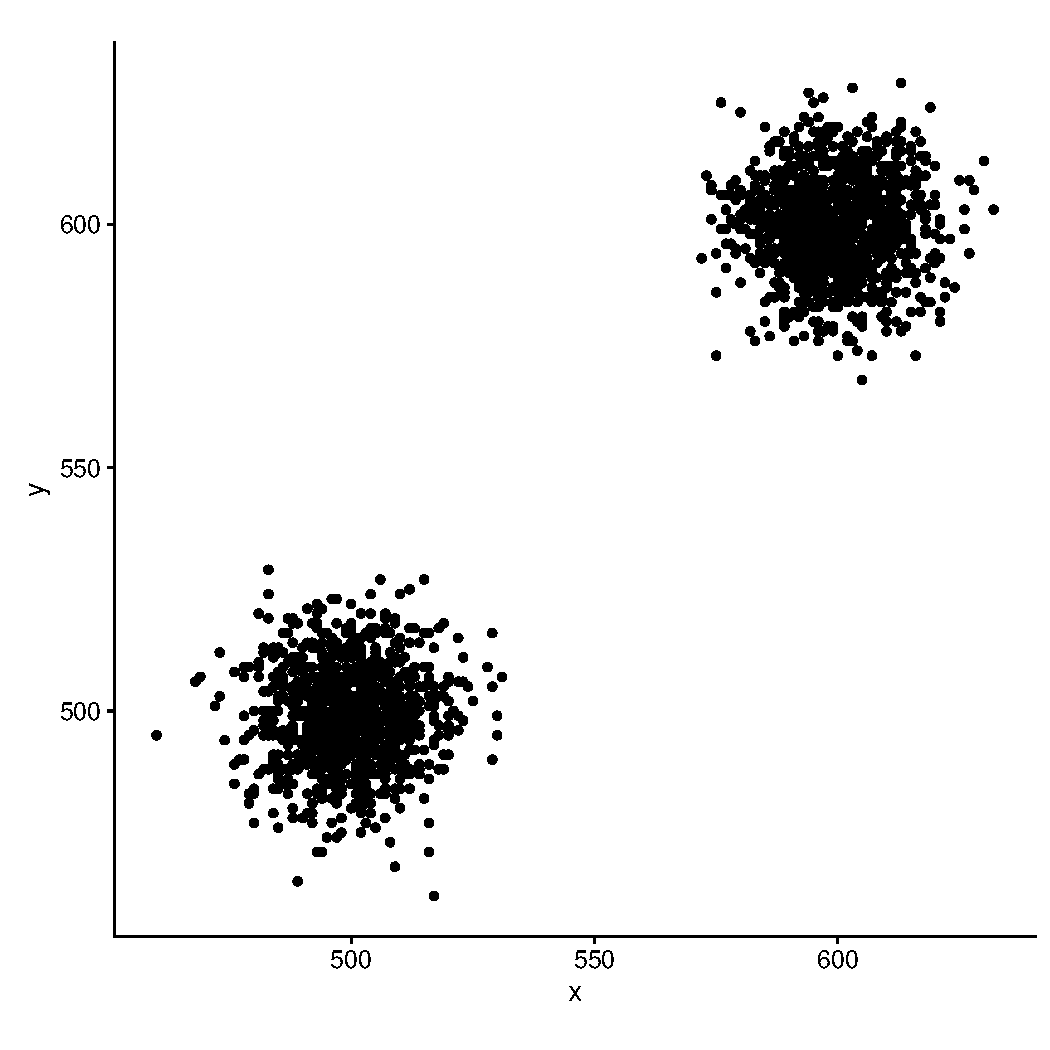
\includegraphics[width=5cm]{./pictures/G2/g2-2-10.pdf}
		\caption*{g2-2-10}
		\label{g2-2-10}
	\end{minipage}
	\begin{minipage}{5cm}
		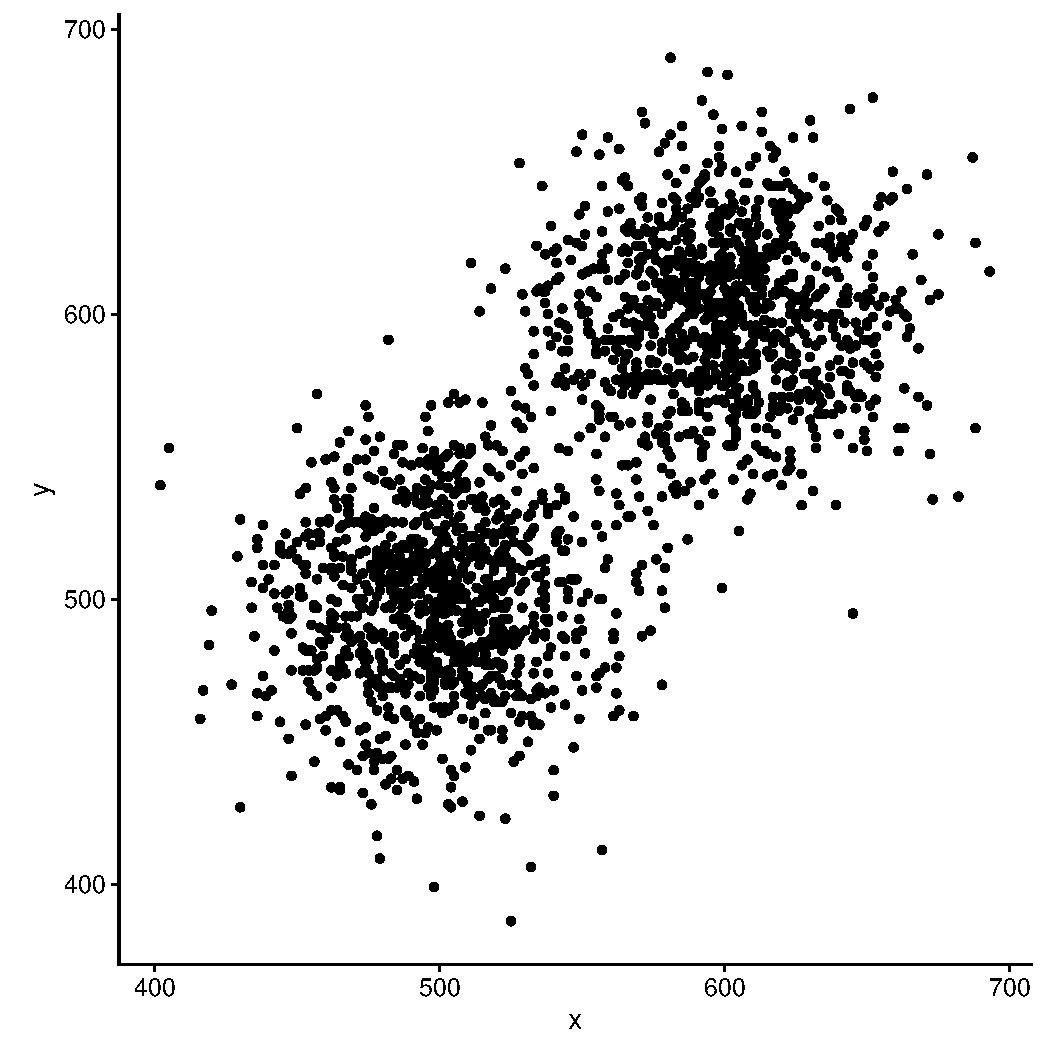
\includegraphics[width=5cm]{./pictures/G2/g2-2-30.pdf}
		\caption*{g2-2-30}
		\label{g2-2-30}
	\end{minipage}
	\\
	\begin{minipage}{5cm}
		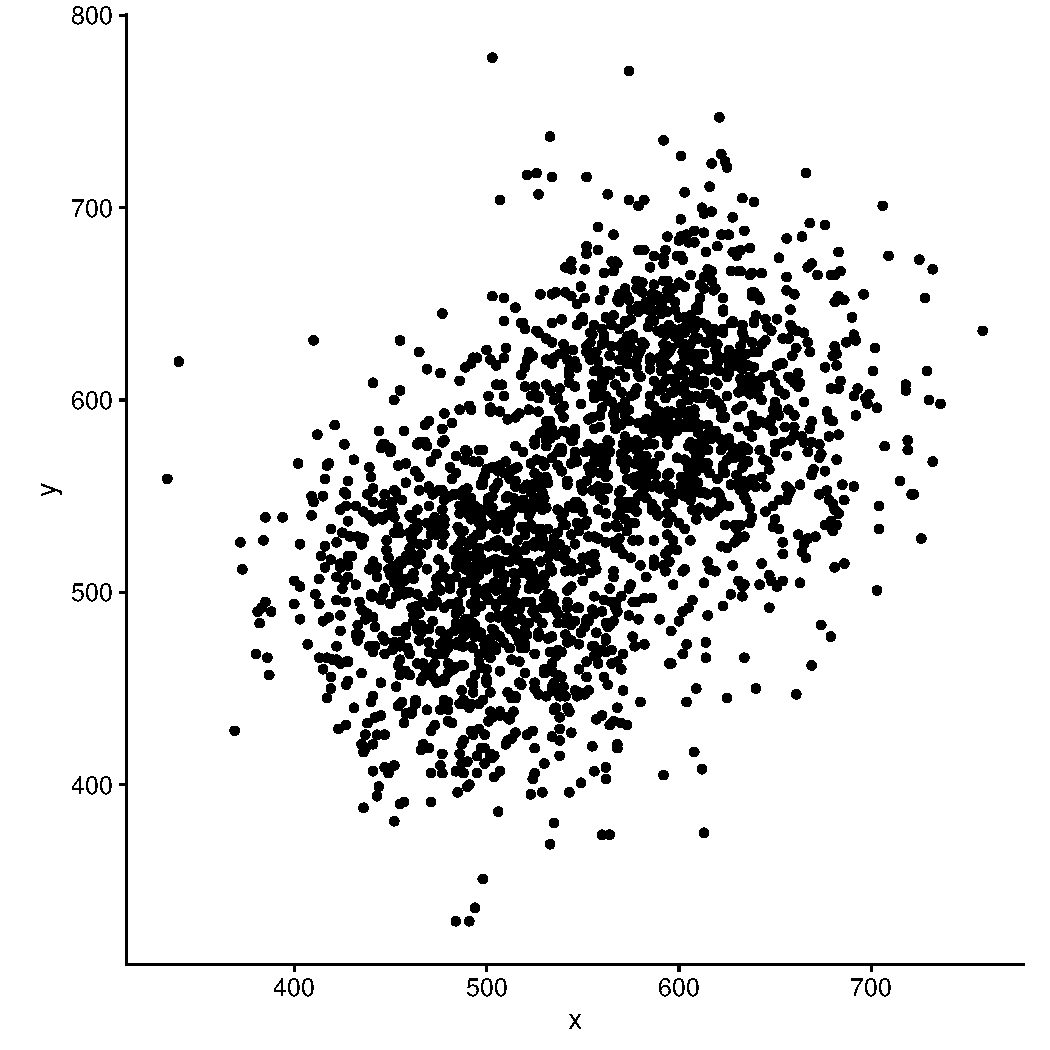
\includegraphics[width=5cm]{./pictures/G2/g2-2-50.pdf}
		\caption*{g2-2-50}
		\label{g2-2-50}
	\end{minipage}
	\begin{minipage}{5cm}
		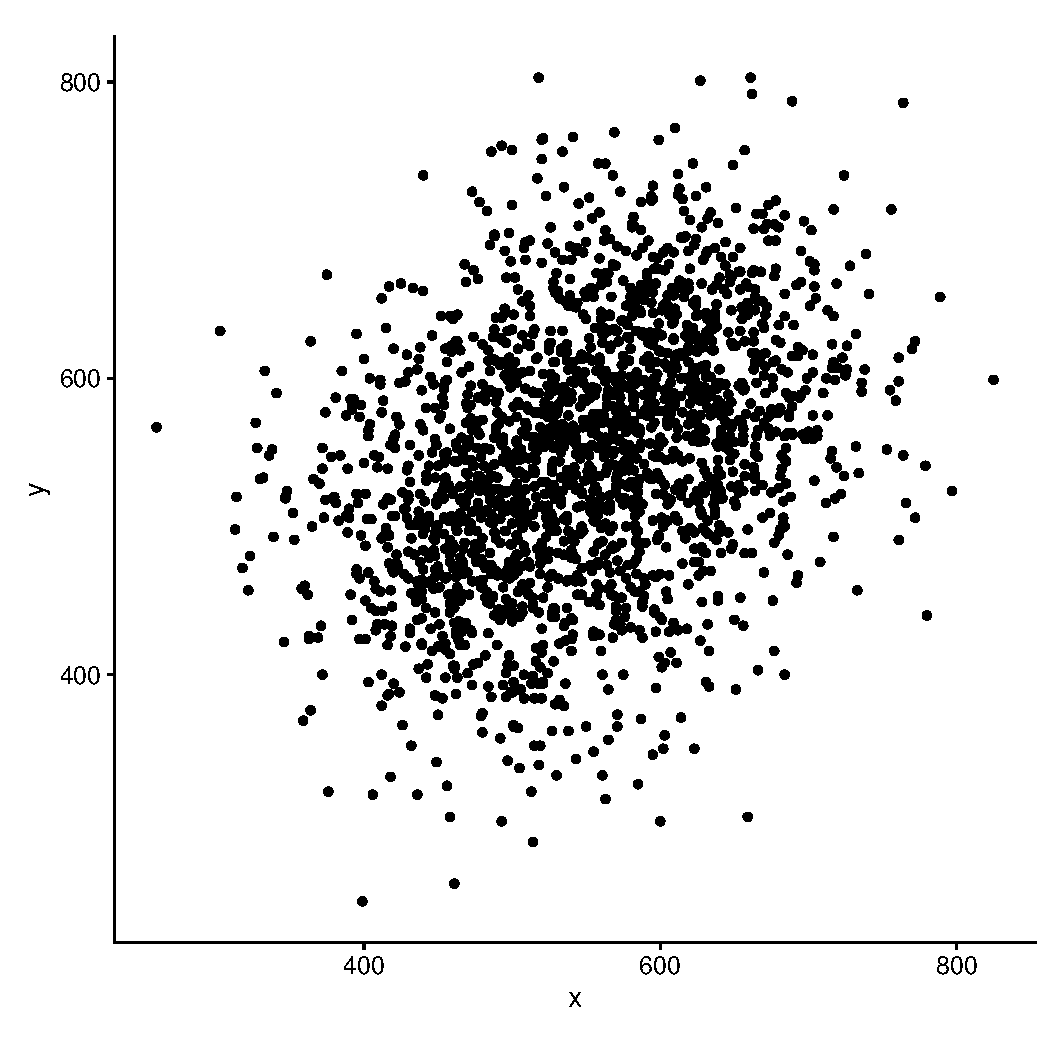
\includegraphics[width=5cm]{./pictures/G2/g2-2-70.pdf}
		\caption*{g2-2-70}
		\label{g2-2-70}
	\end{minipage}
	
	\caption{URL: https://cs.joensuu.fi/sipu/datasets/}
	\label{fig:g2-combined}
\end{figure}

\begin{figure}[H]
	\centering
	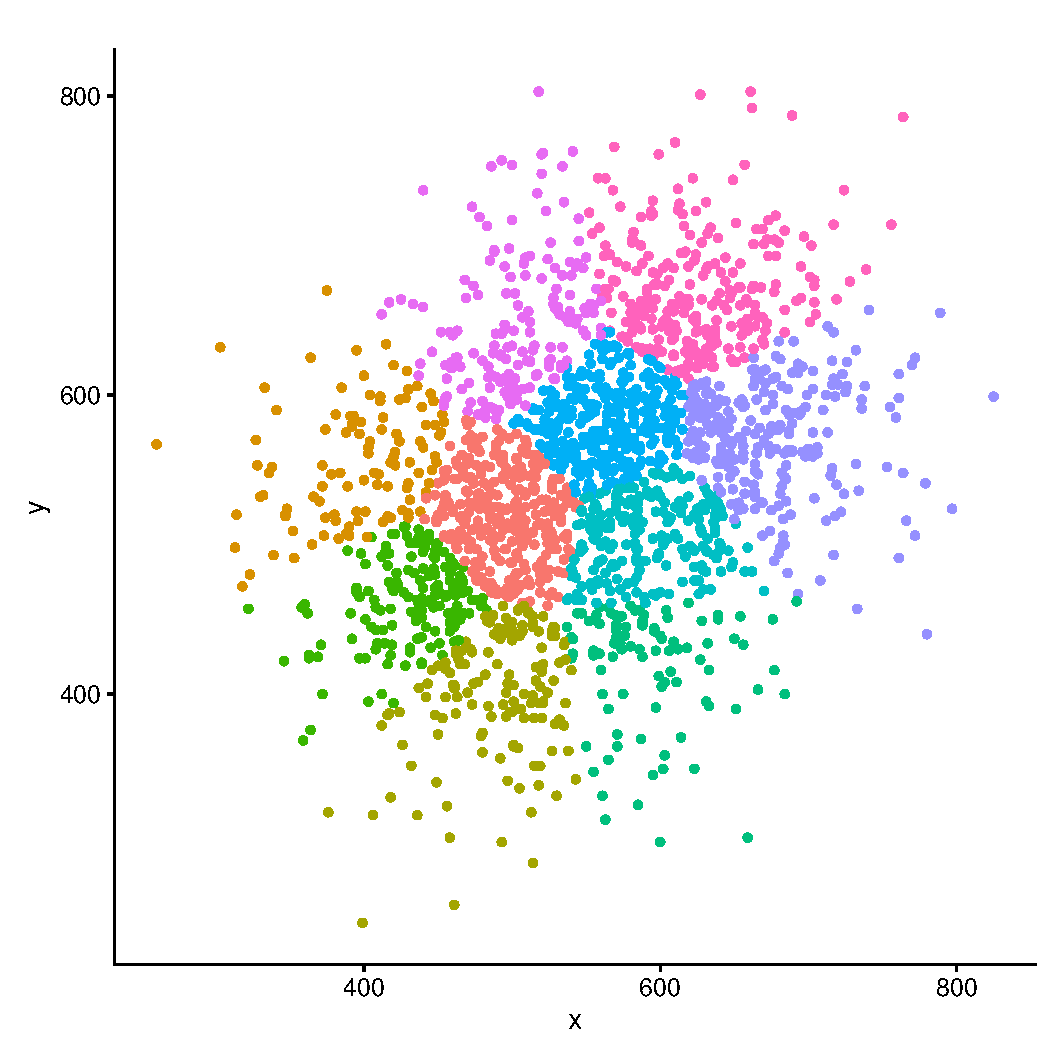
\includegraphics[scale=0.4]{./pictures/G2/g2-2-70-k10.pdf}
	\caption{g2-2-70 clustering with 10 clusters}
	\label{fig:g2-2-70-k10}
\end{figure}
The basic data for a cluster analysis starts with a $n \cdot p$ multivariate data matrix, \texttt{X}, which describes each object to be clustered. The entry $x_{ij}$ gives the value of the \texttt{j}th variable on object \texttt{i}:
\begin{figure}[H]
	\centering
	\[
	\texttt{X}
	=
	\begin{bmatrix}
	x_{11} & x_{12} & \dots & x_{1p} \\
	x_{21} & x_{22} & \dots & \dots \\
	\vdots & \vdots & \vdots & \vdots \\
	x_{n1} & \dots & \dots & x_{np}
	\end{bmatrix}
	\]
	\caption{Multivariate data matrix}
	\label{fig:dataMatrix}
\end{figure}

Many clustering techniques begins by converting \texttt{X} into a symmetric $n \cdot n$ matrix. Both rows and columns represents the objects in the data set. The resulting matrix could be of similarities, dissimilarities or distances between all objects.\\

The formal definition of a cluster can be difficult to give, and it is not clear how a cluster is recognized when displayed in the plane. Looking at figure \ref{shapeDataSets} we have a lot of different types of data sets, which does not have much in common in terms of shapes. Looking at the "two" clusters to the right in the \texttt{Aggregation} set, intuitively these are in fact two clusters, but in some situations it would be more relevant to see them as a single cluster, since they are linked together by a few objects. Looking at the \texttt{path-based2:spiral} set, the clusters are linked together by the neighbors of an object. Dependent on what we are looking for it could be that the objects closest to the center should be in the same cluster. In terms of the \texttt{Zahn's Compound} set it can be hard to determine the outliers. The objects in the lower left corner would intuitively be two clusters. Or, the objects in the middle as a cluster and the ring of objects as outliers. With the two circular clusters(upper left corner) and the square cluster(right side), the clusters could be the dense area around the centers, and outliers around them. Also, the outliers could be members of the clusters. 
\begin{figure}[H]
	\centering
	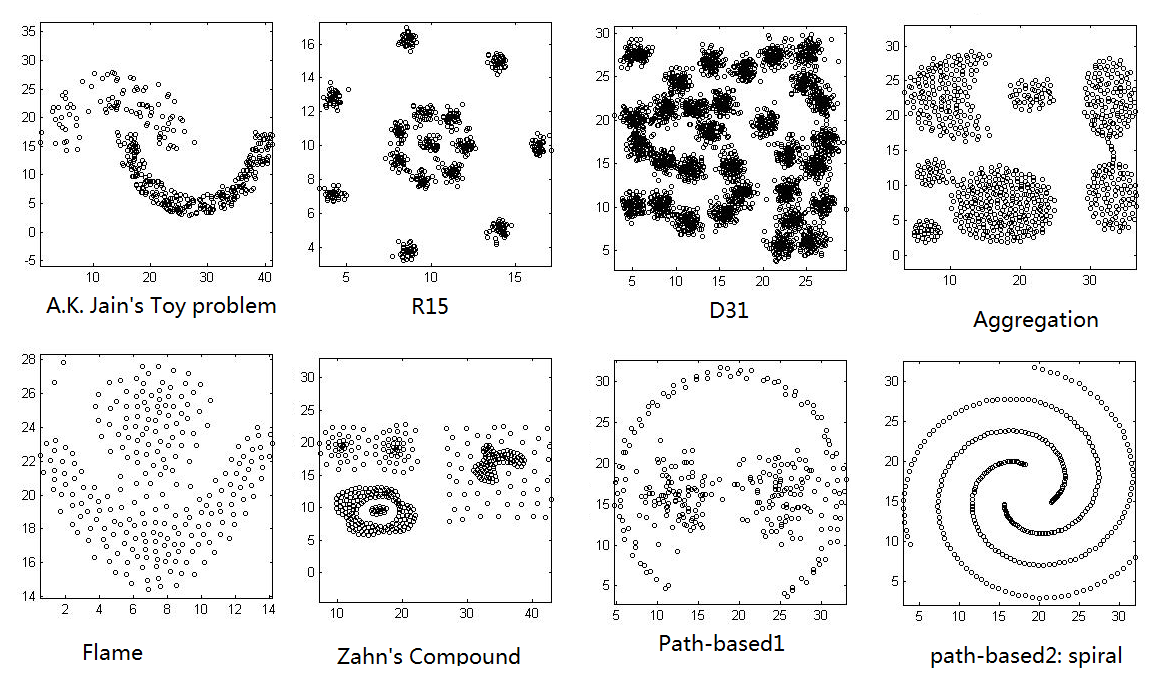
\includegraphics[scale=0.4]{./pictures/shapeDataSet/shapeDataSet.png}
	\caption{Shape Data sets from URL: https://cs.joensuu.fi/sipu/datasets/}
	\label{shapeDataSets}
\end{figure}

Assessing the quality of a clustering can be a challenging task. Clustering is Unsupervised Learning where it is unknown a priori what the best clustering looks like. Many validation techniques requires a \texttt{gold standard} in order to measure the quality. A \texttt{gold standard} to a given dataset is a solution developed by experts. Quality measures that requires a \texttt{gold standard} are Rand Measure, F-measure, Jaccard Index and Dice Index to name a few. One that does not need a gold standard is Sum of Squares which calculates the sum of distances of all objects in a cluster to its centroid. A low value indicates a good clustering, and a high value indicates bad clustering. One problem with Sum of Squares is that a clustering with all objects as it own cluster(singleton clusters) would have a Sum of Squares of 0. Thus, theoretically imply a good clustering, but rarely, if not none, would this ever give any new information.

There are many different algorithms for cluster analysis and which one to use is highly dependent on the dataset. Some of the more known algorithms are \texttt{k-means}, \texttt{hierarchical clustering}, \texttt{Shared Nearest Neighbor}, \texttt{DBSCAN}. \texttt{k-means} is the de-facto standard algorithm for clustering, as it generally performs well. All algorithms takes a set of parameters in order to do the clustering. \texttt{k-means} has one, where \texttt{DBSCAN} has two. Parameter \texttt{k} in \texttt{k-means} is the number of clusters it should return. It can be difficult to determine a single parameter, and increasing the number of parameters exponentially increases the difficulty of setting the parameters. Although, calculating the \texttt{F-ratio} can give a good indication of an optimal \texttt{k} for \texttt{k-means}. In this project we chose \texttt{Transitivity Clustering(TC)}, based on the \texttt{Weighted Transitivity Graph Projection Problem}. F-measure will be used as quality measure. TC and F-measure will be discussed later.


%%%%%%%%%%%%%%%%%%%%%%%%%%%%%%%%%%%%%%%%%%%%%%%%%%
%%%%%%%%%%%%%%%%%%%%%%%%%%%%%%%%%%%%%%%%%%%%%%%%%%
%%%%%%%%%%%%%%%%%%%%%%%%%%%%%%%%%%%%%%%%%%%%%%%%%%
\newpage
\section{Background}
%%%%%%%%%%%%%%%%%%%%%%%%%%%%%%%%%%%%%%%%%%%%%%%%%%
%%%%%%%%%%%%%%%%%%%%%%%%%%%%%%%%%%%%%%%%%%%%%%%%%%
%%%%%%%%%%%%%%%%%%%%%%%%%%%%%%%%%%%%%%%%%%%%%%%%%%

%%%%%%%%%%%%%%%%%%%%%%%%%%%%%%%%%%%%%%%%%%%%%%%%%%
%%%%%%%%%%%%%%%%%%%%%%%%%%%%%%%%%%%%%%%%%%%%%%%%%%
\subsection{Transitivity Clustering}
%%%%%%%%%%%%%%%%%%%%%%%%%%%%%%%%%%%%%%%%%%%%%%%%%%
%%%%%%%%%%%%%%%%%%%%%%%%%%%%%%%%%%%%%%%%%%%%%%%%%%
% article 'Comprehensive cluster analysis with Transitivity Clustering'
% article 'Partitioning biological data with transitivity clustering'
% article 'Large scale clustering of protein sequence with FORCE-A layout based heuristic for weighted cluster editing'

Before going into any details about Transitivity Clustering(TC) we need some basic graph-theoretic definitions.
\begin{description}
	\item[Definitions from 'Extension and Robustness of Transitivity Clustering for Protein...']
\end{description}

\begin{defn}[\texttt{Undirected simple graph}]\label{def:Undirected simple graph}
	An \texttt{undirected simple graph} $G = (V, E)$ consists of a set of nodes V and a set of edges $E \subseteq {V \choose 2}$, where ${V \choose 2}$ denotes the set of two-element subsets of V. The edges are undirected and contains no self-loops or multiple edges between two nodes. \textit{uv} is an unordered par $\{u, v \} \in {V \choose 2}$.
\end{defn}

\begin{defn}[\texttt{Transitive graph}]\label{def:Transitive graph}
	An undirected simple graph $G = (V, E)$ is called \texttt{transitive} 
	\begin{equation*}
	\text{if for all triples } uvw \in {V \choose 3}, uv \in E \text{ and } vw \in E \text{ implies } uw \in E.
	\end{equation*}
\end{defn}

\begin{defn}[\texttt{Weighted Transitive Graph Projection Problem(WTGPP)}]\label{def:WTGPP}
	 Given a set of objects \texttt{V}, a threshold $t \in \mathbb{R}$, and a pairwise similarity function sim: ${V \choose 2} \rightarrow \mathbb{R}$, the graph \textit{G} is defined as
	 \begin{equation}\label{eq:sim above threshold}
	 G = (V, E); \; E = \bigg\{ uv \in {V \choose 2} : \text{sim}(uv) > t\bigg\}
	 \end{equation}
	 The WTGPP is the determination of a transitive graph $G' = (V, E')$ such that there exist no other transitive graph $G'' = (V, E'')$ with $\text{cost}(G \rightarrow G'') < \text{cost}(G \rightarrow G')$. The modification costs are defined as
	 \begin{equation}\label{eq:TC cost function}
		 \text{cost}(G \rightarrow G') := \underbrace{\sum_{uv \in E \backslash E'} | \text{sim}(uv) - t |}_{\text{deletion cost}} + \underbrace{\sum_{uv \in E' \backslash E} | \text{sim}(uv) - t |}_{\text{addition cost}}
	 \end{equation}
\end{defn}

% Briefly write about the steps in the "algorithm" from article 'Comprehensive cluster analysis with trans clust'
% Talk about R package ????? (implementation section ?)

Transitivity Clustering takes one parameter, \textit{t}, which is the threshold for similarities. Following is the steps in Transitivity Clustering: \\
\textbf{Reference: Comprehensive cluster analysis with Transitivity Clustering}
\begin{enumerate}
	\item Model the given pairwise similarity, from the similarity matrix, as a similarity graph, \textit{G}. The nodes corresponds to the objects, with weighted edges as the similarity values.
	
	\item Transform the similarity graph, \textit{G}, into another graph, \textit{G'}, by subtracting the threshold from the edge weights. Subsequently removing those edges with weights below zero, which is the deletion cost for equation \ref{eq:TC cost function}.
	
	\item Transform \textit{G'} into a transitive graph, \textit{G''}, with minimal cost. Thus, in this step we add all edges such that the graph is transitive, which is the addition cost for equation \ref{eq:TC cost function}.
\end{enumerate}
The resulting transitive graph, \textit{G''}, is the clustering solution.


%%%%%%%%%%%%%%%%%%%%%%%%%%%%%%%%%%%%%%%%%%%%%%%%%%
%%%%%%%%%%%%%%%%%%%%%%%%%%%%%%%%%%%%%%%%%%%%%%%%%%
\subsection{Hierarchical Clustering}
%%%%%%%%%%%%%%%%%%%%%%%%%%%%%%%%%%%%%%%%%%%%%%%%%%
%%%%%%%%%%%%%%%%%%%%%%%%%%%%%%%%%%%%%%%%%%%%%%%%%%
% Chapter 4 from Cluster Analysis book
% Look at notes.tex

\begin{defn}[\texttt{Hierarchical Clustering(HC)}]\label{def:hc}
	\textbf{Reference from Unsupervised Learning slides: Hierarchical Clustering}\\
	Builds a nested structural partition $C = 	\{ C_1, \dots, C_k\}$ of \textit{V} such that $\cup_{i = 1}^{k} C_i = V$ and $C_i \neq \emptyset$ $\forall i \in \{1, \dots, k\}$. $\forall \text{ pairs } C_i, C_j$ where $i,j \in \{1, \dots, k\}, i \neq j$, exactly one of the following holds
	\begin{itemize}
		\item $C_i \cap C_j = \emptyset$
		\item $C_i \subset C_j$
		\item $C_j \subset C_i$
	\end{itemize}
\end{defn}

There are two forms of hierarchical Clustering, \texttt{agglomerative} and \texttt{divisive}. Agglomerate starts with \textit{n} clusters, where \textit{n} is the number of objects in the dataset. Joining clusters until one cluster is remaining, where all \textit{n} objects are members. Divisive is the opposite. Starting with one cluster with \textit{n} objects. Splitting the clusters until all clusters are singletons. Thus, all \textit{n} objects represents are cluster. Agglomerative is the most used, as divisive usually is a more expensive procedure. One important feature of hierarchical clustering is that a join or split of clusters are irrevocable, thus cannot be undone. Figure \ref{fig:agglo_vs_div} shows an overview of agglomerative vs. divisive.
\begin{figure}[H]
	\centering
	\includegraphics*[scale=0.4]{./pictures/hc/agglo_vs_div.png}
	\caption{Agglomerative vs. Divisive}
	\label{fig:agglo_vs_div}
\end{figure} 
The steps of joins or splits is often showed as a \texttt{dendrogram}, which is viewed as a tree structure. The root of the tree is the cluster containing all \textit{n} objects. Moving down the tree the nodes represents the clusters which was split from its parent. At the bottom of the tree we have the leafs, where the number of leafs represents all singleton clusters(the \textit{n} objects). The tree can be cut a given height resulting in a clustering solution. Figure \ref{fig:hc example} shows a \texttt{dendrogram} of the tree structure of a HC. The horizontal axis shows all the objects in the dataset. The vertical axis shows the distances between objects and/or clusters. Objects 1 and 2 are joined to a cluster at height 2. These are joined with the remaining objects at height 4, resulting in one cluster holding all objects.
\begin{figure}[H]
	\centering
	\includegraphics*[scale=0.3]{./pictures/hc/hc_example.png}
	\caption{Dendrogram of a Hierarchical Clustering}
	\label{fig:hc example}
\end{figure}

In a typical hierarchical Clustering the size and number of clusters are given by a threshold, much like the one used in \texttt{TC}. Meaning that one iteration can possibly affect all clusters, which either increases or decreases the overall quality. In Figure \ref{fig:hc example} the tree could be cut between height 3-7.5 to obtain a solution containing two clusters.
\\\textbf{Might not be the right section explaining about cutting the tree to gain optimal solution(Dynamic tree cut)}\\
In Figure \ref{fig:hc quality example} we could cut the tree between height 3-7.5 and we would get a solution containing two clusters. One issue in terms of quality is that, the optimal clustering solution could have the clusters {5, 2}, {3, 6, 1},  {7} and {4, 0}. Making a horizontal cut in the tree, it would be impossible to obtain this solution. However, if it was possible to make a dynamic tree cut, the optimal solution could in fact be obtained. The solution can be made by cutting the tree in three different heights. First cut is between 2.5 and 7.5 to obtain the cluster {5, 1}. Cutting between height 2.0 and 3.0, obtaining cluster {3, 6, 1}. The last cut is between 2.5 and 3, giving the last clusters {7} and {4, 0}.
\begin{figure}[H]
	\centering
	\includegraphics*[scale=0.4]{./pictures/hc/hc_quality_example.png}
	\caption{}
	\label{fig:hc quality example}
\end{figure}


%%%%%%%%%%%%%%%%%%%%%%%%%%%%%%%%%%%%%%%%%%%%%%%%%%
%%%%%%%%%%%%%%%%%%%%%%%%%%%%%%%%%%%%%%%%%%%%%%%%%%
\subsection{Cluster Validation}
%%%%%%%%%%%%%%%%%%%%%%%%%%%%%%%%%%%%%%%%%%%%%%%%%%
%%%%%%%%%%%%%%%%%%%%%%%%%%%%%%%%%%%%%%%%%%%%%%%%%%
% Section 'cluster comparison' from article 'Large scale clustering of protein sequence with FORCE-A layout based heuristic for weighted cluster editing'
% Look at source.tex in articles folder

%%%%%%%%%%%%%%%%%%%%%%%%%%%%%%%%%%%%%%%%%%%%%%%%%%
%%%%%%%%%%%%%%%%%%%%%%%%%%%%%%%%%%%%%%%%%%%%%%%%%%
\subsection{Multidimensional Scaling}
%%%%%%%%%%%%%%%%%%%%%%%%%%%%%%%%%%%%%%%%%%%%%%%%%%
%%%%%%%%%%%%%%%%%%%%%%%%%%%%%%%%%%%%%%%%%%%%%%%%%%

%%%%%%%%%%%%%%%%%%%%%%%%%%%%%%%%%%%%%%%%%%%%%%%%%%
%%%%%%%%%%%%%%%%%%%%%%%%%%%%%%%%%%%%%%%%%%%%%%%%%%
\subsection{GAP Statistics}
%%%%%%%%%%%%%%%%%%%%%%%%%%%%%%%%%%%%%%%%%%%%%%%%%%
%%%%%%%%%%%%%%%%%%%%%%%%%%%%%%%%%%%%%%%%%%%%%%%%%%
% This is what is used for the reasoning of the randomization

%%%%%%%%%%%%%%%%%%%%%%%%%%%%%%%%%%%%%%%%%%%%%%%%%%
%%%%%%%%%%%%%%%%%%%%%%%%%%%%%%%%%%%%%%%%%%%%%%%%%%
%%%%%%%%%%%%%%%%%%%%%%%%%%%%%%%%%%%%%%%%%%%%%%%%%%
\newpage
\section{Method}
%%%%%%%%%%%%%%%%%%%%%%%%%%%%%%%%%%%%%%%%%%%%%%%%%%
%%%%%%%%%%%%%%%%%%%%%%%%%%%%%%%%%%%%%%%%%%%%%%%%%%
%%%%%%%%%%%%%%%%%%%%%%%%%%%%%%%%%%%%%%%%%%%%%%%%%%

%%%%%%%%%%%%%%%%%%%%%%%%%%%%%%%%%%%%%%%%%%%%%%%%%%
%%%%%%%%%%%%%%%%%%%%%%%%%%%%%%%%%%%%%%%%%%%%%%%%%%
\subsection{Assessing best clustering}
%%%%%%%%%%%%%%%%%%%%%%%%%%%%%%%%%%%%%%%%%%%%%%%%%%
%%%%%%%%%%%%%%%%%%%%%%%%%%%%%%%%%%%%%%%%%%%%%%%%%%
% This might be too similar with the sections under introduction ?

%%%%%%%%%%%%%%%%%%%%%%%%%%%%%%%%%%%%%%%%%%%%%%%%%%
%%%%%%%%%%%%%%%%%%%%%%%%%%%%%%%%%%%%%%%%%%%%%%%%%%
\subsection{Randomization approach 1}
%%%%%%%%%%%%%%%%%%%%%%%%%%%%%%%%%%%%%%%%%%%%%%%%%%
%%%%%%%%%%%%%%%%%%%%%%%%%%%%%%%%%%%%%%%%%%%%%%%%%%
% Look at notes.tex

%%%%%%%%%%%%%%%%%%%%%%%%%%%%%%%%%%%%%%%%%%%%%%%%%%
%%%%%%%%%%%%%%%%%%%%%%%%%%%%%%%%%%%%%%%%%%%%%%%%%%
\subsection{Randomization approach 2}
%%%%%%%%%%%%%%%%%%%%%%%%%%%%%%%%%%%%%%%%%%%%%%%%%%
%%%%%%%%%%%%%%%%%%%%%%%%%%%%%%%%%%%%%%%%%%%%%%%%%%
% Look at notes.tex

%%%%%%%%%%%%%%%%%%%%%%%%%%%%%%%%%%%%%%%%%%%%%%%%%%
%%%%%%%%%%%%%%%%%%%%%%%%%%%%%%%%%%%%%%%%%%%%%%%%%%
\subsection{Randomization approach 3}
%%%%%%%%%%%%%%%%%%%%%%%%%%%%%%%%%%%%%%%%%%%%%%%%%%
%%%%%%%%%%%%%%%%%%%%%%%%%%%%%%%%%%%%%%%%%%%%%%%%%%

%%%%%%%%%%%%%%%%%%%%%%%%%%%%%%%%%%%%%%%%%%%%%%%%%%
%%%%%%%%%%%%%%%%%%%%%%%%%%%%%%%%%%%%%%%%%%%%%%%%%%
\subsection{Randomization approach 4}
%%%%%%%%%%%%%%%%%%%%%%%%%%%%%%%%%%%%%%%%%%%%%%%%%%
%%%%%%%%%%%%%%%%%%%%%%%%%%%%%%%%%%%%%%%%%%%%%%%%%%

%%%%%%%%%%%%%%%%%%%%%%%%%%%%%%%%%%%%%%%%%%%%%%%%%%
%%%%%%%%%%%%%%%%%%%%%%%%%%%%%%%%%%%%%%%%%%%%%%%%%%
\subsection{Results for randomizations}
%%%%%%%%%%%%%%%%%%%%%%%%%%%%%%%%%%%%%%%%%%%%%%%%%%
%%%%%%%%%%%%%%%%%%%%%%%%%%%%%%%%%%%%%%%%%%%%%%%%%%
% Write about the results from the randomizations, and reasons to try other approaches.

%%%%%%%%%%%%%%%%%%%%%%%%%%%%%%%%%%%%%%%%%%%%%%%%%%
%%%%%%%%%%%%%%%%%%%%%%%%%%%%%%%%%%%%%%%%%%%%%%%%%%
\subsection{Short about the implementation / tools}
%%%%%%%%%%%%%%%%%%%%%%%%%%%%%%%%%%%%%%%%%%%%%%%%%%
%%%%%%%%%%%%%%%%%%%%%%%%%%%%%%%%%%%%%%%%%%%%%%%%%%

%%%%%%%%%%%%%%%%%%%%%%%%%%%%%%%%%%%%%%%%%%%%%%%%%%
%%%%%%%%%%%%%%%%%%%%%%%%%%%%%%%%%%%%%%%%%%%%%%%%%%
%%%%%%%%%%%%%%%%%%%%%%%%%%%%%%%%%%%%%%%%%%%%%%%%%%
\newpage
\section{Conclusion}
%%%%%%%%%%%%%%%%%%%%%%%%%%%%%%%%%%%%%%%%%%%%%%%%%%
%%%%%%%%%%%%%%%%%%%%%%%%%%%%%%%%%%%%%%%%%%%%%%%%%%
%%%%%%%%%%%%%%%%%%%%%%%%%%%%%%%%%%%%%%%%%%%%%%%%%%

%%%%%%%%%%%%%%%%%%%%%%%%%%%%%%%%%%%%%%%%%%%%%%%%%%
%%%%%%%%%%%%%%%%%%%%%%%%%%%%%%%%%%%%%%%%%%%%%%%%%%
%%%%%%%%%%%%%%%%%%%%%%%%%%%%%%%%%%%%%%%%%%%%%%%%%%
\newpage
\section{References}
%%%%%%%%%%%%%%%%%%%%%%%%%%%%%%%%%%%%%%%%%%%%%%%%%%
%%%%%%%%%%%%%%%%%%%%%%%%%%%%%%%%%%%%%%%%%%%%%%%%%%
%%%%%%%%%%%%%%%%%%%%%%%%%%%%%%%%%%%%%%%%%%%%%%%%%%





\end{document}
